\cleardoublepage
\counterwithout{figure}{section}
\counterwithout{table}{section} 
\counterwithout{equation}{section}
\counterwithin{figure}{chapter}
\counterwithin{table}{chapter} 
\counterwithin{equation}{chapter}


\chapter{Introduction}
\label{sec:problemstellung}
 Only in Germany more than 1 Million teeth are replaced annually.
 And the most popular crown material is Zirconia. However, but Zirconia in its pure form is plain white so coloring the crown is necessary.Dentist are using such a shade guide for a side-by-side comparison to determine the color and the shade of the teeth.One can observe that there are 4 color groups A B C and D and each of these colors have 4 shades coded with the numbers from 1 to 4. Where 1 is the least and 4 is the most saturated shade for each color. 
 
 \begin{figure}[h]
 	\centering
 	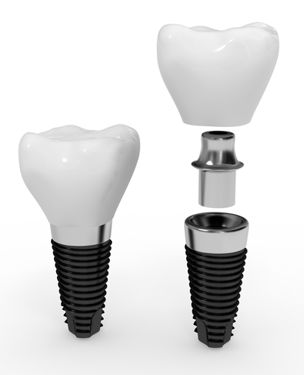
\includegraphics[width=0.4\textwidth]{grafiken/implant.png}
 	\caption{Iam in altera philosophiae parte}
 	\label{fig:bild1}
 \end{figure}

\chapter{State of the Research}
\label{sec:stand_forschung}
\section{Contra quos omnis}
Contra quos omnis dicendum breviter existimo. Quamquam philosophiae quidem vituperatoribus satis responsum est eo libro, quo a nobis philosophia defensa et collaudata est, cum esset accusata et vituperata ab Hortensio. qui liber cum et tibi probatus videretur et iis, quos ego posse iudicare arbitrarer, plura suscepi veritus ne movere hominum studia viderer, retinere non posse. \citet{autor1} qui autem, si maxime hoc placeat, moderatius tamen id volunt fieri, difficilem quandam temperantiam postulant in eo, quod semel admissum coerceri reprimique non potest, ut propemodum iustioribus utamur illis, qui omnino avocent a philosophia, quam his, qui rebus infinitis modum constituant in reque eo meliore, quo maior sit, mediocritatem desiderent. \citep{autor2}

\subsection{Sapientiam perveniri}
Sive enim ad sapientiam perveniri potest, non paranda nobis solum ea, sed fruenda etiam [sapientia] est; sive hoc difficile est, tamen nec modus est ullus investigandi veri, nisi inveneris, et quaerendi defatigatio turpis est, cum id, quod quaeritur, sit pulcherrimum. etenim si delectamur, cum scribimus, quis est tam invidus, qui ab eo nos abducat? sin laboramus, quis est, qui alienae modum statuat industriae? nam ut Terentianus Chremes non inhumanus, qui novum vicinum non vult 'fodere aut arare aut aliquid ferre denique' -- non enim illum ab industria, sed ab inliberali labore deterret --, sic isti curiosi, quos offendit noster minime nobis iniucundus labor.

\subsection{Graecis expressas}
\label{sec:freiheitsgrad_eines_getriebes}
Iis igitur est difficilius satis facere, qui se Latina scripta dicunt contemnere. in quibus hoc primum est in quo admirer, cur in gravissimis rebus non delectet eos sermo patrius, cum idem fabellas Latinas ad verbum e Graecis expressas non inviti legant. quis enim tam inimicus paene nomini Romano est, qui Ennii Medeam aut Antiopam Pacuvii spernat aut reiciat, quod se isdem Euripidis fabulis delectari dicat, Latinas litteras oderit?



\section{A quibus tantum dissenti}
\label{sec:grundlagen_für_die_kinematischen_betrachtungen}
A quibus tantum dissentio, ut, cum Sophocles vel optime scripserit Electram, tamen male conversam Atilii mihi legendam putem, de quo Lucilius: 'ferreum scriptorem', verum, opinor, scriptorem tamen, ut legendus sit. rudem enim esse omnino in nostris poetis aut inertissimae segnitiae est aut fastidii delicatissimi. mihi quidem nulli satis eruditi videntur, quibus nostra ignota sunt. an 'Utinam ne in nemore . . .' nihilo minus legimus quam hoc idem Graecum, quae autem de bene beateque vivendo a Platone disputata sunt, haec explicari non placebit Latine?

\chapter{State of the Technology}
\label{sec:stand_technik}
On the left side you can see a cutout of a lab card. Dentists mark different areas of the crown with different colors from the guide for the technicians.
And on the right side are the tasks of a dental technician, which are mainly:
-Milling 
-Manually coloring using a brush
-furnacing to burn the color to the Zirconia
-and lastly polishing for a natural look.
And the coloring part is the process, on which this thesis is focused 


\chapter{Review of the State of the Art and Technology}
\label{sec:kritik_stand_technik}
s